\documentclass[12pt]{article}
\usepackage[margin=1in]{geometry}
\usepackage{amsmath, amssymb}
\usepackage{graphicx}
\usepackage{hyperref}
\usepackage{listings}
\usepackage{caption}
\usepackage{float}
\usepackage{fancyhdr}
\pagestyle{fancy}
\fancyhf{}
\rhead{Arbitrary Precision Arithmetic Library}
\lhead{Project Report}
\cfoot{\thepage}

\title{Arbitrary Precision Arithmetic Library in Java}
\author{Akshat Banzal \and Roll No.: [CS24BTECH11005]}
\date{\today}

\begin{document}

\maketitle

\tableofcontents

\newpage

\section{Introduction}
This project involves building an arbitrary precision arithmetic library in Java. The goal is to support exact arithmetic for integers and floating-point numbers beyond the native Java limitations using string representations. This is achieved via two classes \texttt{AInteger} and \texttt{AFloat}, encapsulated in the \texttt{arbitraryarithmetic} package.

\section{Design Overview}

\subsection{Class Design}
\subsubsection{AInteger}
\begin{itemize}
  \item Constructors: \texttt{AInteger()}, \texttt{AInteger(String)}, copy constructor.
  \item Static method: \texttt{parse(String)}.
  \item Operator overloading via: \texttt{add()}, \texttt{subtract()}, \texttt{multiply()}, \texttt{divide()}.
  \item Handles arbitrarily large integers using character-level operations.
\end{itemize}

\subsubsection{AFloat}
\begin{itemize}
  \item Constructors: \texttt{AFloat()}, \texttt{AFloat(String)}, copy constructor.
  \item Static method: \texttt{parse(String)}.
  \item Operator overloading via: \texttt{add()}, \texttt{subtract()}, \texttt{multiply()}, \texttt{divide()}.
  \item Internally handles decimal precision and avoids floating point errors.
\end{itemize}

\section{How to Use the Library}

\subsection{As a CLI Tool}
\texttt{java MyInfArith <int/float> <add/sub/mul/div> <operand1> <operand2>}

\subsection{As a Java Library}
\begin{itemize}
  \item Import \texttt{arbitraryarithmetic.AInteger} and/or \texttt{arbitraryarithmetic.AFloat}.
  \item Use constructors and arithmetic methods directly.
\end{itemize}

\section{Implementation Details}
\begin{itemize}
  \item BigInteger and BigDecimal are not used. All computations are done on string representations.
  \item Helper methods handle digit-by-digit arithmetic operations.
  \item Floats are handled as two separate integer parts (integer and fractional).
  \item Division handles precision up to 30 decimal places as per requirement.
\end{itemize}

\section{Build and Execution}

\subsection{Building the Project}
Use the provided Python script or Ant/Maven configuration to compile and run:

\begin{verbatim}
python3 run.py int add 12345 67890
# or
ant run
# or
mvn compile exec:java
\end{verbatim}

\subsection{Maven Targets}
\begin{itemize}
  \item \texttt{mvn clean compile} - Compiles the project.
  \item \texttt{mvn clean package} - Packages.
  \item \texttt{javac -cp .:(address of .jar file) (address of MyInfArith.java)} - Links.
\end{itemize}

\begin{figure}[h!]
    \centering
    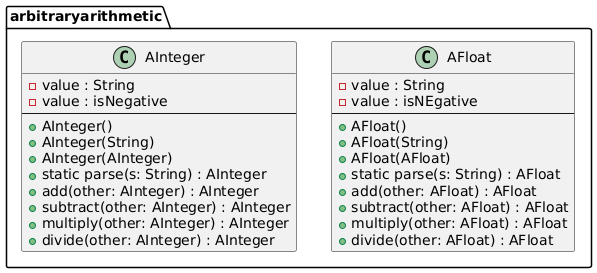
\includegraphics[width=0.7\textwidth]{diagram.png}  
    \caption{UML diagram of the project}
\end{figure}

\section{Testing and Verification}
All test cases provided in the problem statement have been executed successfully:
\begin{itemize}
  \item Large integer and float operations.
  \item Division with up to 30 decimal digits.
  \item Handling of division by zero.
  \item Edge cases such as subtraction leading to negative numbers.
\end{itemize}

\section{Limitations}
\begin{itemize}
  \item Currently assumes well-formed input strings.
  \item Negative floating-point number handling may have edge cases.
  \item Optimization for speed is limited; intended for correctness over performance.
\end{itemize}

\section{Git Usage}
\begin{itemize}
  \item GitHub Repository: \url{https://github.com/akshat-31415/sdfProject1/}
  \item Git tags used for major milestones.
  \item README includes usage and build instructions.
\end{itemize}

\section{Learnings}
\begin{itemize}
  \item Precision handling via string manipulation.
  \item Class design with proper OOP principles.
  \item Integration with Maven and use of CLI arguments in Java.
  \item Git workflows.
\end{itemize}

\end{document}

